\chapter{Research Questions and Proposed Architecture}\label{RQ}

\section{Research Questions}\label{sec:rqs}

This thesis investigates the feasibility, reproducibility, and ecosystem reliability of automated declarative environment generation for computer science education. To guide the empirical inquiry, three central Research Questions (RQs) are formulated:

\begin{enumerate}
	\item \textbf{RQ1 (Agentic Synthesis Accuracy):} Can an AI agent accurately infer system-level dependencies from natural language assignment instructions or unconfigured source code to automatically generate valid, reproducible \texttt{flake.nix} environments?
	\item \textbf{RQ2 (Clean-Container Reproducibility):} To what extent do Nix Flake environments that pass local validation reproduce and support headless coursework tasks in a fresh Linux container without the authoring machine's files, configuration, or prior evaluation state?
	\item \textbf{RQ3 (Classroom Deployment Reliability):} To what extent can Nix Flake environments provide a dependable foundation for classroom use, and what operational constraints and risk trade-offs shape that dependability?
\end{enumerate}

\section{Proposed Solution: The AI-Assisted Flake Synthesis Architecture}\label{chap:solution}

To bridge the gap between complex declarative configurations and educational usability, we propose an automated environment synthesis pipeline. Rather than forcing instructors or students to master the Nix DSL language, our framework delegates the composition, package resolution, and verification of Nix Flakes to an autonomous agent harness.

The end-to-end architecture comprises of the following steps (illustrated at a high level in Figure~\ref{fig:pipeline-overview}):
\begin{enumerate}
	\item \textbf{Requirement Ingestion (Figure~\ref{fig:pipeline-ingestion}):} Natural language assignment specifications or unconfigured assignment codebases are analyzed to extract inferred toolchains, language runtimes, and system-level libraries.
	\item \textbf{Specialized Agent Skill Scaffolding and Live Package Retrieval:} A custom agent skill provides domain-specific prompting, curated templates, and reference schemas, while the agent queries a Model Context Protocol (MCP) server that reaches out to trusted sources of information.
	\item \textbf{Deterministic Closed-Loop Verification:} Generated \texttt{flake.nix} files are evaluated via native Nix commands. If syntax or dependency errors occur, the compiler diagnostics are fed back into the agent harness for iterative self-correction.
	\item \textbf{Output Artifacts and Runtime Deployment:} A \texttt{flake.nix} file is written alongside a cryptographically pinned \texttt{flake.lock} file, immediately activating a reproducible developer shell.
\end{enumerate}

\begin{figure}[htbp]
	\centering
	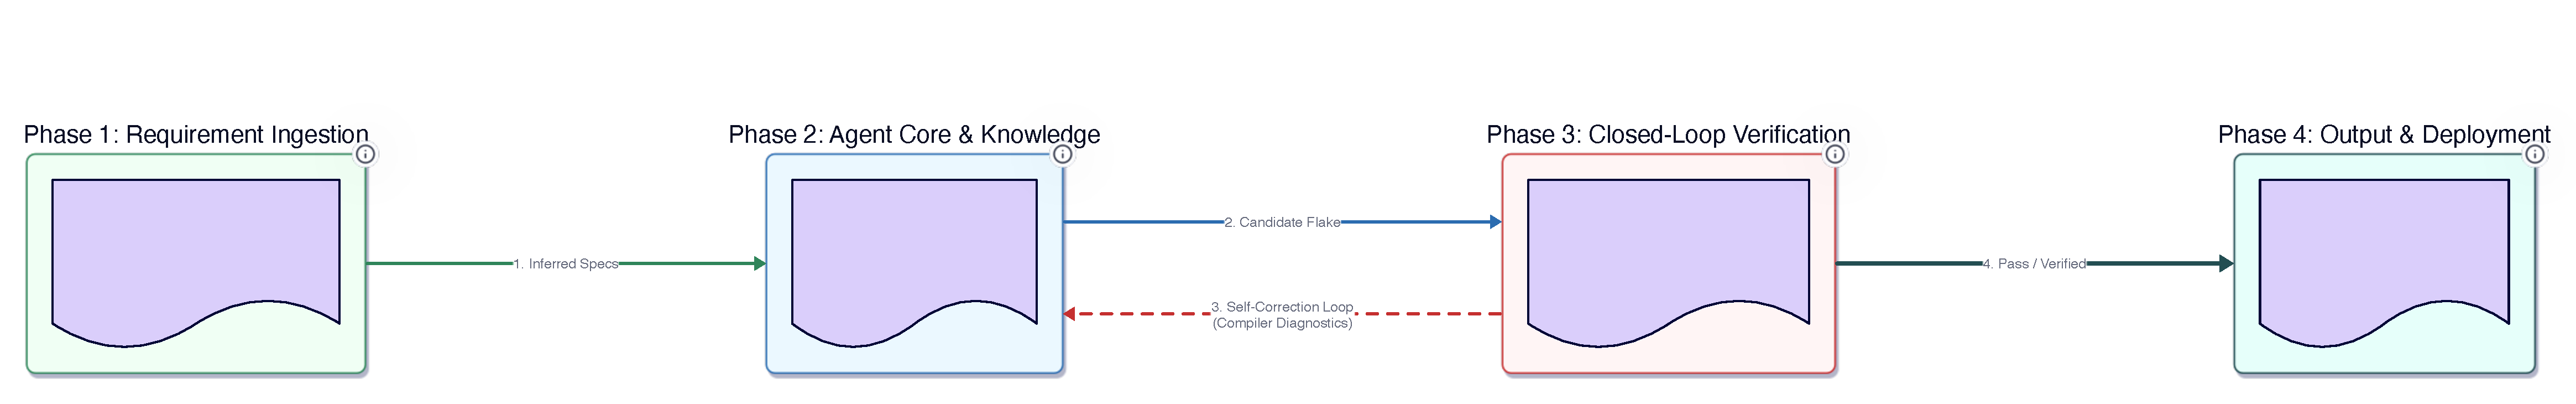
\includegraphics[width=\linewidth,height=0.38\textheight,keepaspectratio]{Figures/pipeline_overview.pdf}
	\caption{High-Level End-to-End Architecture of the Autonomous \texttt{flake.nix} Synthesis Pipeline}
	\label{fig:pipeline-overview}
\end{figure}

\begin{figure}[htbp]
	\centering
	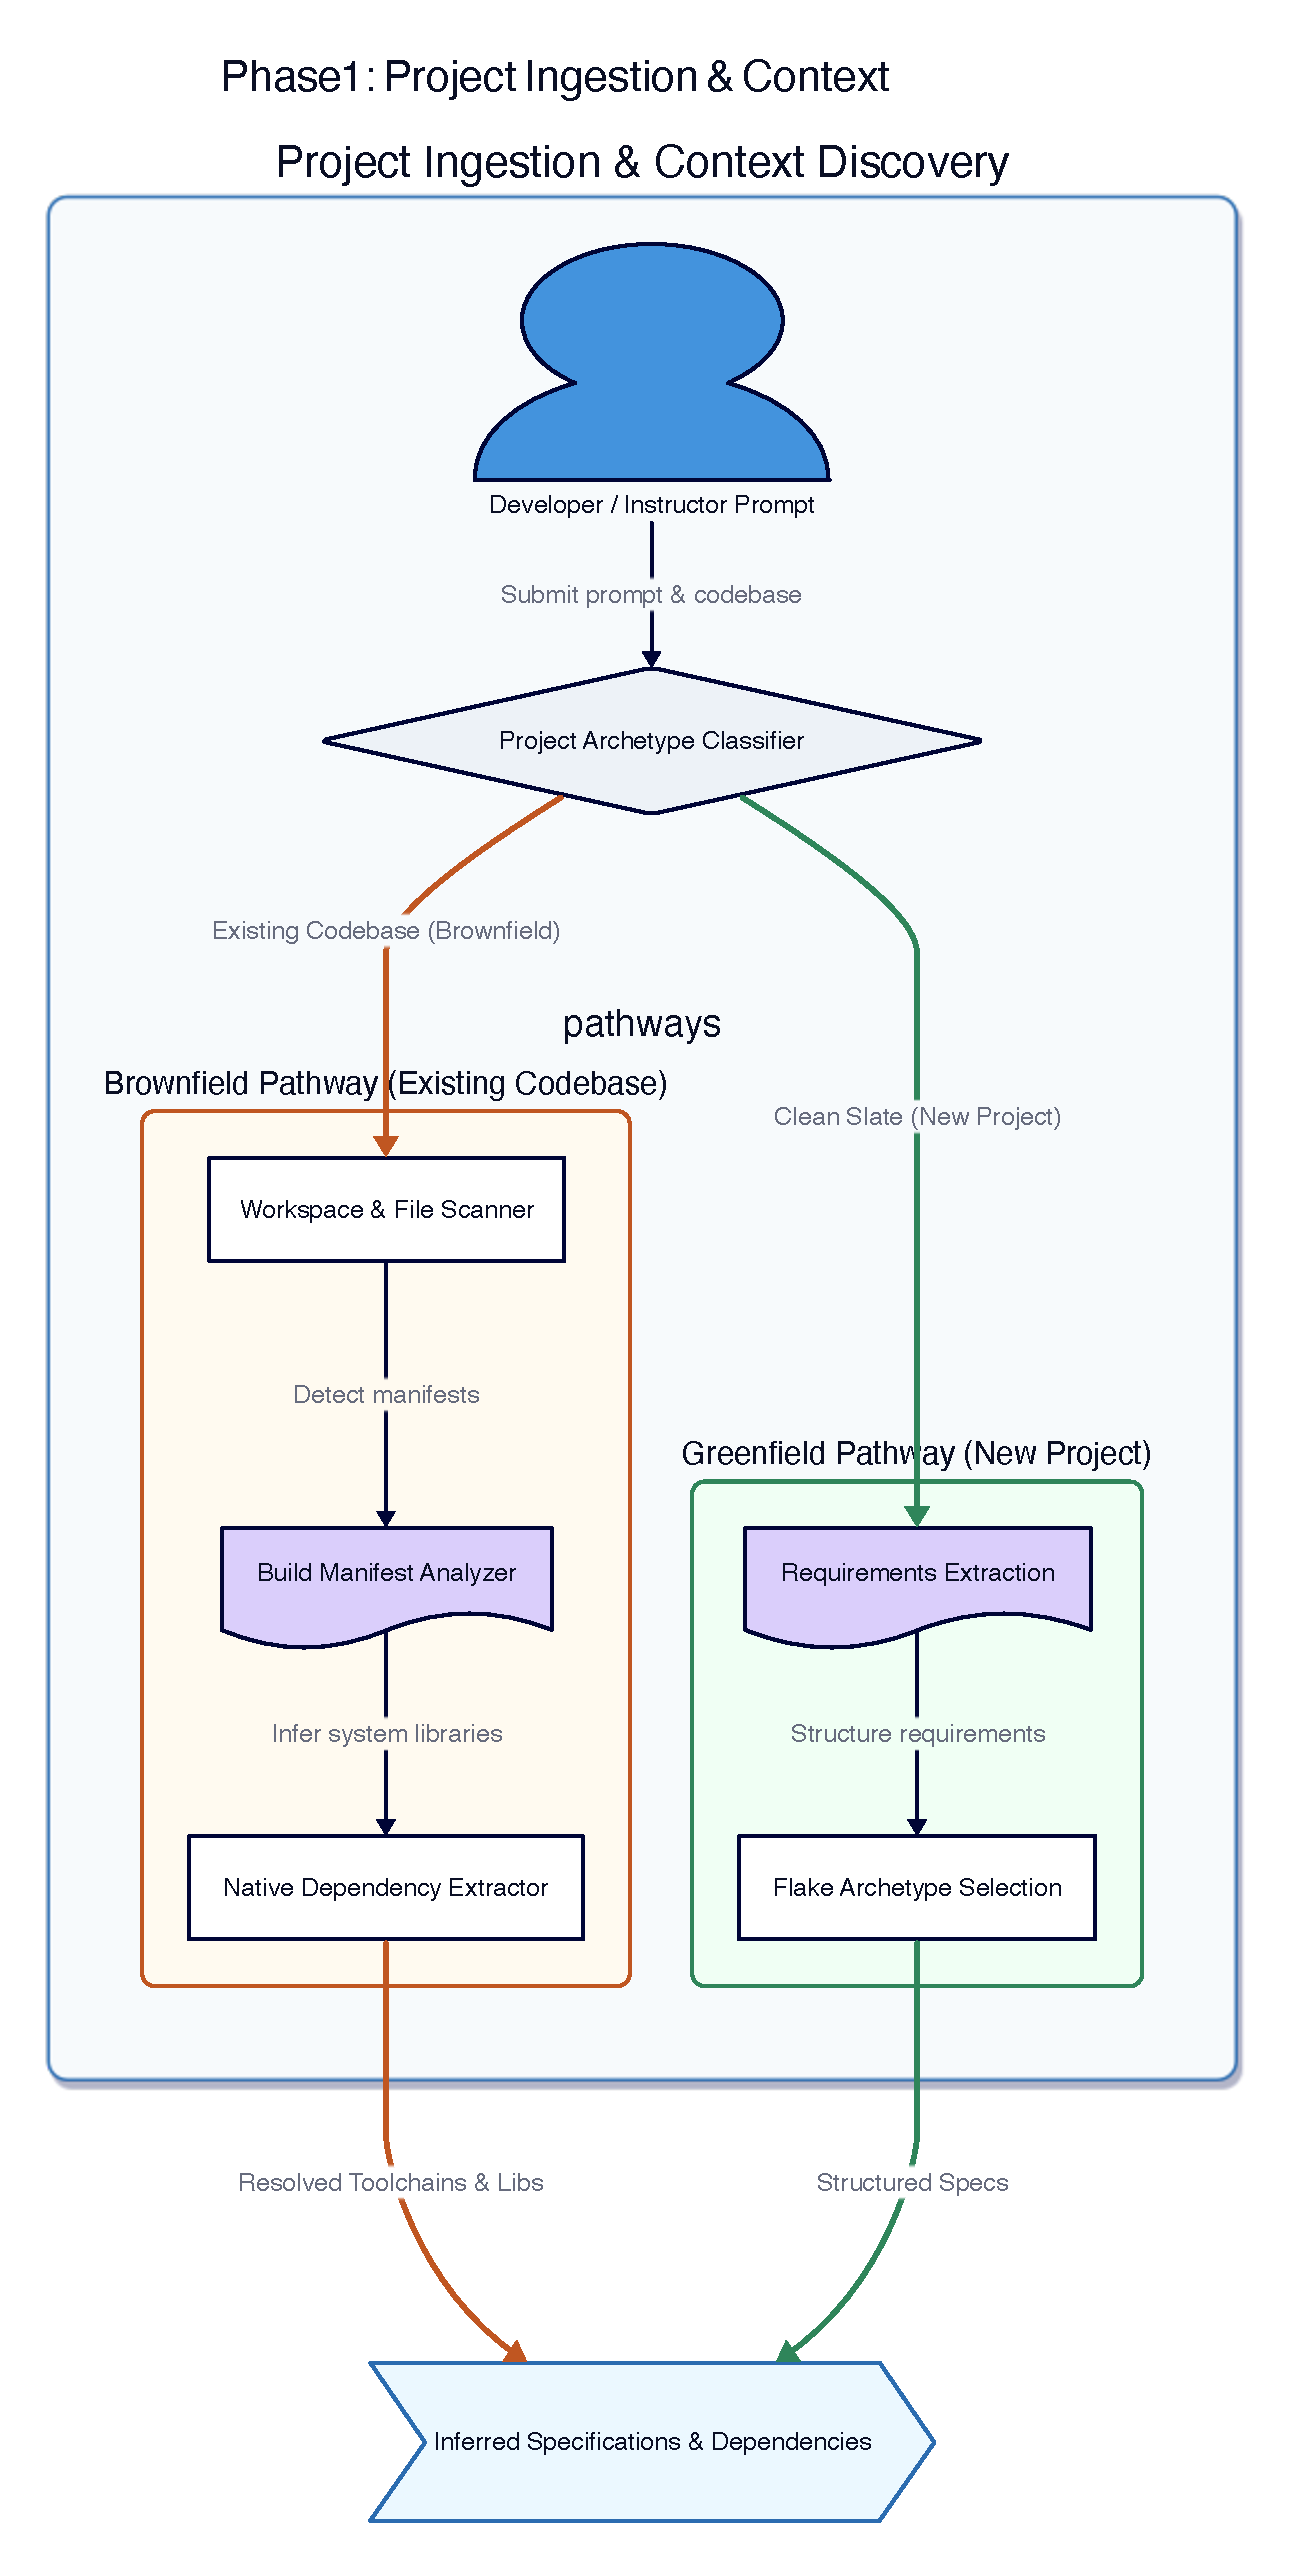
\includegraphics[width=0.9\linewidth,height=0.42\textheight,keepaspectratio]{Figures/pipeline_1_ingestion.pdf}
	\caption{Phase 1: Project Ingestion and Context Discovery Subsystem Across Greenfield and Brownfield Projects}
	\label{fig:pipeline-ingestion}
\end{figure}


\chapter{Experimental Methodology and Test Setup}\label{chap:testing}

\section{Agentic Flake Synthesis Test Design}

Synthesizing flake.nix configuration files requires navigating a purely functional domain-specific language. To eliminate the cognitive overhead of learning Nix syntax and package semantics, we evaluated how effectively modern agents can synthesize valid \texttt{flake.nix} files.

The criteria for passing is as follows:
\begin{itemize}
	\item A \texttt{flake.nix} is generated
	\item Static code analysis via \texttt{nix flake check} passes
	\item Declared dependencies are present in \texttt{\$PATH} after invoking \texttt{nix develop}
\end{itemize}

Antigravity cli, \texttt{agy} and \texttt{codex} were 2 agent harnesses used for testing

Gemini 3.8 Flash with medium reasoning was the default model used with agy
GPT 5.6 was used for

\subsection{Real-Time Package Retrieval via MCP-NixOS}\label{subsec:mcp-nixos}

The Nix Packages collection (\texttt{nixpkgs}) represents one of the largest open-source package repositories in existence. At the time of this research, \texttt{nixpkgs} hosts over 139,008 packages distributed across 1,044 distinct package sets. Because Nixpkgs evolves rapidly with daily upstream commits, static LLM training data is inherently prone to package name mismatches, deprecated attribute paths, and package hallucinations~\cite{ImportingPhantomsMeasuring}.

Recent studies by authors analyzing package hallucinations demonstrate that less popular programming languages suffer significantly higher hallucination frequencies due to the relative scarcity of examples in public pre-training datasets~\cite{ImportingPhantomsMeasuring}. To eliminate this vulnerability, we integrated \texttt{mcp-nixos}, a high-performance FastMCP server that exposes live querying capabilities to the agent harness. The server communicates directly with the Elasticsearch backend powering \texttt{search.nixos.org}, enabling the agent to execute real-time searches across official packages, options, and configuration schemas. By querying \texttt{mcp-nixos}, the agent dynamically verifies exact package attribute names before committing them to the synthesized \texttt{flake.nix} specification.

\subsection{Agent Harness and Model Configurations}

To systematically evaluate synthesis performance, the experimental framework will be tested with the Antigravity CLI agent harness.

Experiments were evaluated across two models: Google Gemini~3.8 Flash and GPT-OSS 120B, with medium reasoning effort.

An automated Python test runner was developed to execute test suites, capture agent tool call telemetry, stream shell outputs, and record execution success metrics.

\subsection{Input Dataset Curation}

Because benchmark datasets for declarative Nix environments did not exist, we constructed an evaluation benchmark representing standard computer science course curricula. The evaluation suite consists of synthetic assignment prompts and starter repositories divided into two distinct curriculum tracks:

\begin{enumerate}
	\item \textbf{Software Development Track:} Curated assignments focusing on systems programming, web engineering, and software construction. These prompts require toolchains such as C++ (GCC/Clang, CMake, Make), Rust (Cargo, rustc), and full-stack Python/Node.js environments.
	\item \textbf{Data Science Track:} Curated coursework requiring complex scientific libraries, interpreted runtimes, and external mathematical packages, including Python (NumPy, SciPy, Pandas, PyTorch), R programming environments, and Jupyter notebook kernels.
\end{enumerate}

These two tracks capture diverse dependencies. While software development projects prioritize native compilation toolchains, data science projects introduce intricate native shared library bindings (such as BLAS, LAPACK, and libstdc++), which often cause severe dependency conflicts on student machines.

\subsection{Input Data Format}

The input data is stored as a json file. Each input contains the following attributes:

\begin{figure}[htbp]
	\begin{lstlisting}
  {
    "track": "...",
    "instruction": "...",
    "dependency": "...",
  }
	\end{lstlisting}
	\caption{Input Data Format}
	\label{fig:input-data-format}
\end{figure}

Where track is either computer science or data science. \texttt{instruction} is the natural language that an instructor might provide. \texttt{dependecy} is a list of executables that should be present when a student invokes \texttt{nix develop}.

\subsection{Specialized Agent Skill Design}\label{subsec:agent-skill}

An agent skill represents a structured, reusable capability module that transforms a general-purpose language model into a specialized domain expert~\cite{AgentSkills,lingAgentSkillsDataDriven2026}. Because generating Nix Flakes for varied academic courses is a recurrent task, relying purely on unstructured zero-shot prompts produces high variance and erratic tool utilization.

We designed a custom agent skill named \texttt{course-flake-generator}. The skill exposes YAML frontmatter metadata that allows agent harnesses to index and match the skill against user instructions:

\begin{figure}[htbp]
	\begin{lstlisting}
---
name: course-flake-generator
description: Generates a nix flake file based on an instructor's requirements or with a provided project folder with source code and other artifacts. Use when creating, generating, or configuring a Nix flake (flake.nix) for course assignments, lab environments, or software projects from specifications, natural language instructions, or existing codebases. Don't use for non-Nix environments, simple shell scripts, or general documentation generation.
---
	\end{lstlisting}
	\caption{Course Flake Generator Metadata}
	\label{fig:course-flake-generator-metadata}
\end{figure}

The internal directory structure of the custom agent skill follows standardized agentic skill packaging conventions:

\begin{figure}[htbp]
	\begin{lstlisting}
.
├── assets
│   ├── flake-devshell.template.nix
│   └── mcp-servers.template.json
├── references
│   ├── flake-patterns.md
│   ├── inferring-requirements.md
│   └── mcp-nixos.md
├── scripts
│   ├── detect-project-requirements.py
│   ├── query-nixos.py
│   └── validate-flake.py
└── SKILL.md
	\end{lstlisting}
	\caption{Custom Skill Filetree Structure}
	\label{fig:custom-skill-filetree}
\end{figure}

The \texttt{assets/} directory bundles validated boilerplate templates for \texttt{devShells} across multi-architecture systems. The \texttt{references/} directory supplies documentation outlining common Nix idiomatic patterns and troubleshooting heuristics. The \texttt{scripts/} directory provides standalone Python utilities that execute deterministic requirement detection and local flake validation. According to Ling et~al.~\cite{lingAgentSkillsDataDriven2026}, providing modular templates and clear reference bounds significantly improves behavioral consistency and task adherence in autonomous agents.

\subsection{Evaluation Metrics and Pass@K Formulation}

To rigorously evaluate the synthesis capabilities of the agents, we adapted the standard Pass@$k$ formulation from code generation literature. A synthesized environment is considered successful if and only if it satisfies three automated validation stages:
\begin{enumerate}
	\item \textbf{Grammar and Evaluation Validity:} The command \texttt{nix flake check} evaluates without syntax or attribute resolution errors.
	\item \textbf{Build and Realization Determinism:} The command \texttt{nix develop --command <test-cmd>} successfully enters the ephemeral shell and resolves all declared binaries on the \texttt{PATH}.
	\item \textbf{Functional Task Execution:} The assignment source code builds and passes its unit test suite inside the synthesized \texttt{devShell}.
\end{enumerate}

Pass@K where we generate $n >= k$ samples per task. For our testing purposes, we set

\[
	\text{pass}@k := \underset{\text{Problems}}{\mathbb{E}} \left[ 1 - \frac{\binom{n-c}{k}}{\binom{n}{k}} \right]
\]


\section{Clean-Container Reproducibility Methodology}

RQ2 evaluates whether a successful local validation actually transfers to an environment that has none of the authoring host's files, shell configuration, or prior evaluation state. The replay cohort contains only RQ1 trial artifacts that passed the three-stage local verifier and include both a generated \texttt{flake.nix} and its \texttt{flake.lock}. This design evaluates the reproducibility of fixed artifacts rather than re-running the agent or permitting it to repair configurations during the clean-container test.

Each validation stage is replayed in a newly created, unmounted Linux Docker container containing Nix. The harness streams a compressed copy of the trial into the container and extracts it into container-local temporary storage; no project directory or host Nix store is mounted. The container is discarded when the stage finishes, so no writable state is shared by stages or trials. Network access remains available so that a first-use environment can retrieve its pinned inputs and binary-cache artifacts; availability failures are recorded separately from configuration failures.

The guest-side verifier executes the following stages in order:
\begin{enumerate}
	\item \textbf{Locked Flake Evaluation:} \texttt{nix flake check} evaluates the generated flake with lock-file writes disabled.
	\item \textbf{Development-Shell Activation:} \texttt{nix develop --command true} verifies that the development shell can be realized and activated.
	\item \textbf{Required Tool Availability:} Each executable listed in the original RQ1 dependency assertion is checked with \texttt{command -v} inside the development shell.
	\item \textbf{Headless Task Execution:} A curated per-task command set verifies applicable language runtimes, builds, dependency synchronization, or test commands. Graphical editor workflows, interactive credentials, and persistent database-service administration are excluded because they cannot be assessed consistently by a headless guest.
\end{enumerate}

The principal metric is the clean-container reproduction rate: the proportion of eligible RQ1-passing trials that complete every applicable container-side stage. Failures are classified as flake-evaluation failures, shell-activation failures, missing dependencies, functional task failures, or infrastructure failures. For each trial, the harness records the source-run identifier, container image digest and system architecture, Nix version, command exit codes, standard output and error logs, and stage durations. These artifacts make it possible to distinguish a defective generated environment from a transient container or upstream package-source failure.

\section{Ecosystem Reliability and Trust Methodology}

RQ3 examines the operational dependencies that remain after a flake has passed local and clean-container validation. A pinned \texttt{flake.lock} separates ordinary classroom activation from dependency maintenance: students should activate a committed lock file rather than invoke \texttt{nix flake update} during a lab. Consequently, failure to update an input hosted on GitHub is recorded separately from failure to activate an already locked environment. This distinction prevents a transient source-host outage from being mischaracterized as a failure of a fixed course environment.

The assessment considers four conditions. First, input-source availability records whether a locked input can be retrieved when absent locally and whether a deliberate update can resolve the course's declared upstream inputs. Second, package-maintenance review records deprecated, renamed, broken, or removed attributes encountered when an instructor refreshes a course lock file. Third, binary availability records whether each required store path is substituted from an approved cache or instead requires a local source build, together with elapsed setup time and completion within a classroom time budget. Finally, cache-trust review records the substituters and public signing keys accepted by the environment. Nix verifies cached paths against trusted keys; adding a third-party cache can improve availability, but it also expands the set of entities trusted to provide course binaries~\cite{dolstraNixSafePolicyFree}.

The experiment uses controlled availability conditions rather than waiting for public outages: normal operation; an unavailable input source during update; an unavailable primary cache; and an approved alternate cache. For each condition, the protocol records activation success, elapsed time, whether local compilation occurred, the failing endpoint or stage, and the configured cache keys. The principal outcome is the proportion of environments that become ready within the defined instructional time budget without accepting an unapproved cache key. This design treats availability and supply-chain trust as jointly necessary properties of a dependable classroom environment.

\chapter{Empirical Results and Analysis}\label{chap:results}

\section{Flake Synthesis Accuracy and Model Comparison}\label{sec:model-results}

Our experimental evaluation revealed notable variations across model architectures, curriculum domains, and the presence of specialized agent skills. In baseline evaluations conducted without the custom agent skill, general-purpose LLMs exhibited a strong tendency toward imperative fallbacks. Specifically, when operating on a macOS test host, models frequently attempted to install missing packages imperatively via Homebrew (\texttt{brew install}), failing to produce a declarative \texttt{flake.nix} file entirely.

With the introduction of the \texttt{course-flake-generator} skill, synthesis adherence improved substantially. The agent successfully adhered to the declarative flake pattern for over 85\% of standard software development prompts. However, curriculum domain complexity strongly influenced outcomes. While the Software Development track achieved high Pass@1 rates, prompts in tfhe Data Science track exhibited higher initial failure rates. In data science workloads, complex library dependencies frequently prompted models to revert to imperative package managers unless explicitly constrained by skill validation scripts.

\section{Tool Invocation and Telemetry Analysis}

By aggregating and analyzing the frequency distribution of agent tool invocations, we identified significant insights into model reasoning behaviors. Removing the agent's access to mcp-nixos mcp server showed suprising results. The agent was able to synthesize by invoking nix cli commands to retrieve enough information about the requirements prompted.

	\textbf{Nix CLI vs. MCP-NixOS Server Utilization:} Gemini~3.8 Flash, configured with medium reasoning effort, demonstrated a pronounced preference for invoking native Nix command-line inspection tools (such as \texttt{nix-env -qaP} and \texttt{nix search}) rather than routing requests through the dedicated \texttt{mcp-nixos} server.
	      Because Gemini's training data incorporates extensive documentation on standard Nix package conventions, the model .

	\textbf{Knowledge Cutoffs and Package Drift:} Gemini~3 has a documented pre-training knowledge cutoff of March 2026. In instances where upstream Nixpkgs deprecated specific package attributes between 2025 and 2026, models relying solely on internal knowledge produced evaluation errors.

\section{Clean-Container Reproducibility Results - TODO}

The clean-container replay will report the reproduction rate for eligible RQ1-passing artifacts, disaggregated by curriculum track and failure category. These results will identify which locally valid flakes remain functional in a fresh Nix container and which dependencies or task requirements escape the initial host-side validation.

\section{Ecosystem Reliability and Trust Results - TODO}

RQ3 results will report readiness within the instructional time budget under normal operation, unavailable input-source, unavailable-primary-cache, and approved-alternate-cache conditions. The analysis will separate locked-environment activation from \texttt{flake update}, identify package-maintenance failures encountered during lock refresh, and report source-build fallback and cache-key decisions without conflating an availability failure with an invalid flake.

\subsection{Security Considerations}

\subsection{Nix Caches}

Nix normally realizes a required store path by downloading a signed substitute from a binary cache; when no acceptable substitute is available, it may instead build the path locally from source. This fallback preserves the possibility of realization but can be unsuitable for a classroom when compilation exceeds the time available for a laboratory session. Thus, cache availability is an operational reliability concern rather than merely a performance optimization.

Nix can use additional binary caches, known as substituters, to improve availability. A substitute is accepted only when its signature corresponds to a configured trusted public key. This signature mechanism provides an integrity boundary, but adding an external cache and its key is a supply-chain decision: it authorizes that cache operator to provide binaries that students will execute. A course should therefore use only institutionally approved cache URLs and keys, document them in the course environment, and avoid asking students to trust arbitrary caches~\cite{dolstraNixSafePolicyFree}.


\section{Ecosystem Reliability in Classroom Deployment}

Nix Flakes make dependencies explicit, but they do not eliminate dependence on the services and maintainers that supply those dependencies. Nixpkgs inputs are commonly fetched from GitHub. A GitHub outage can therefore prevent an instructor from refreshing a flake input and can prevent a new machine from fetching a locked input that is not already available locally. These are different operational events: a committed lock file protects ordinary coursework from unintended version drift, whereas updating the lock file remains an instructor maintenance activity that depends on upstream availability.

The breadth of Nixpkgs also creates a maintenance risk. Package definitions may become deprecated, renamed, broken, or removed when upstream software is abandoned or when no contributor continues to maintain its Nix expression. Pinning a course environment provides a stable term-level target, but it does not remove the need to review package availability before the next term or before updating a lock file. Instructors should therefore establish a refresh schedule, retain a tested lock file for the current offering, and identify a supported alternative when a course depends on a narrowly maintained package.

Finally, binary-cache misses turn an availability event into a student-facing time cost. A departmental cache or an approved external substituter can reduce that risk, but it must be governed as part of the course's trusted computing base. RQ3 consequently evaluates reliability as a combination of input availability, maintained package definitions, bounded setup time, and an explicit cache-trust policy rather than as a property of the \texttt{flake.nix} file alone.
